% !TeX root = ../main.tex
\chapter{Archival Ordinance Scan Defect Plates}
\label{app:ocr_defect_plates}

This appendix documents the physical degradation artifacts, typography variations, and optical scanning defects encountered across historical Davao City local ordinances (1945--2026), accompanied by empirical OCR transcription error comparisons.

\section{Historical Ordinance Degradation Typology}
\label{sec:app_ocr_degradation_typology}

Physical ordinance records preserved in the Sangguniang Panlungsod archives exhibit severe mechanical and chemical degradation patterns spanning four distinct legislative eras. Table~\ref{tab:app_scan_defect_typology} classifies the primary defect categories affecting automated optical character recognition.

\begin{table}[htbp]
    \centering
    \small
    \caption{Archival Document Degradation Typology for Davao City Ordinances}
    \label{tab:app_scan_defect_typology}
    \begin{tabular}{lp{3.5cm}p{4cm}p{4.2cm}}
        \toprule
        \textbf{Era} & \textbf{Primary Medium} & \textbf{Physical Defects} & \textbf{Downstream OCR Impact} \\
        \midrule
        1945--1971 & Mechanical typewriter (low-gsm pulp paper) & Variable strike pressure, ribbon ink depletion, paper yellowing & Broken character glyphs, faint punctuation, merged ascenders \\
        1972--1986 & Carbon paper duplicates and cyclostyle mimeographs & Ink feathering, background bleed-through, character haloing & Severe false-positive character insertions, elevated Word Error Rate (WER) \\
        1987--2000 & Early photocopies and dot-matrix printouts & Binding hole punch shadows, toner spatter, affine page skew & Section heading truncation, obscured marginal section numbering \\
        2001--2026 & Digital laser prints and modern PDF scans & Clean digital typography, occasional skewed scanner bed feeds & Near-zero character error rate; isolated line wrap misalignments \\
        \bottomrule
    \end{tabular}
\end{table}

\section{Archival Scan Defect Plates}
\label{sec:app_visual_defect_plates}

Figure~\ref{fig:app_archival_degradation_plate} illustrates typical physical degradation patterns observed in archival enactments from the 1950s and 1960s, demonstrating carbon bleed-through, faded mechanical ribbon strikes, and binding margin occlusions.

\begin{figure}[htbp]
    \centering
    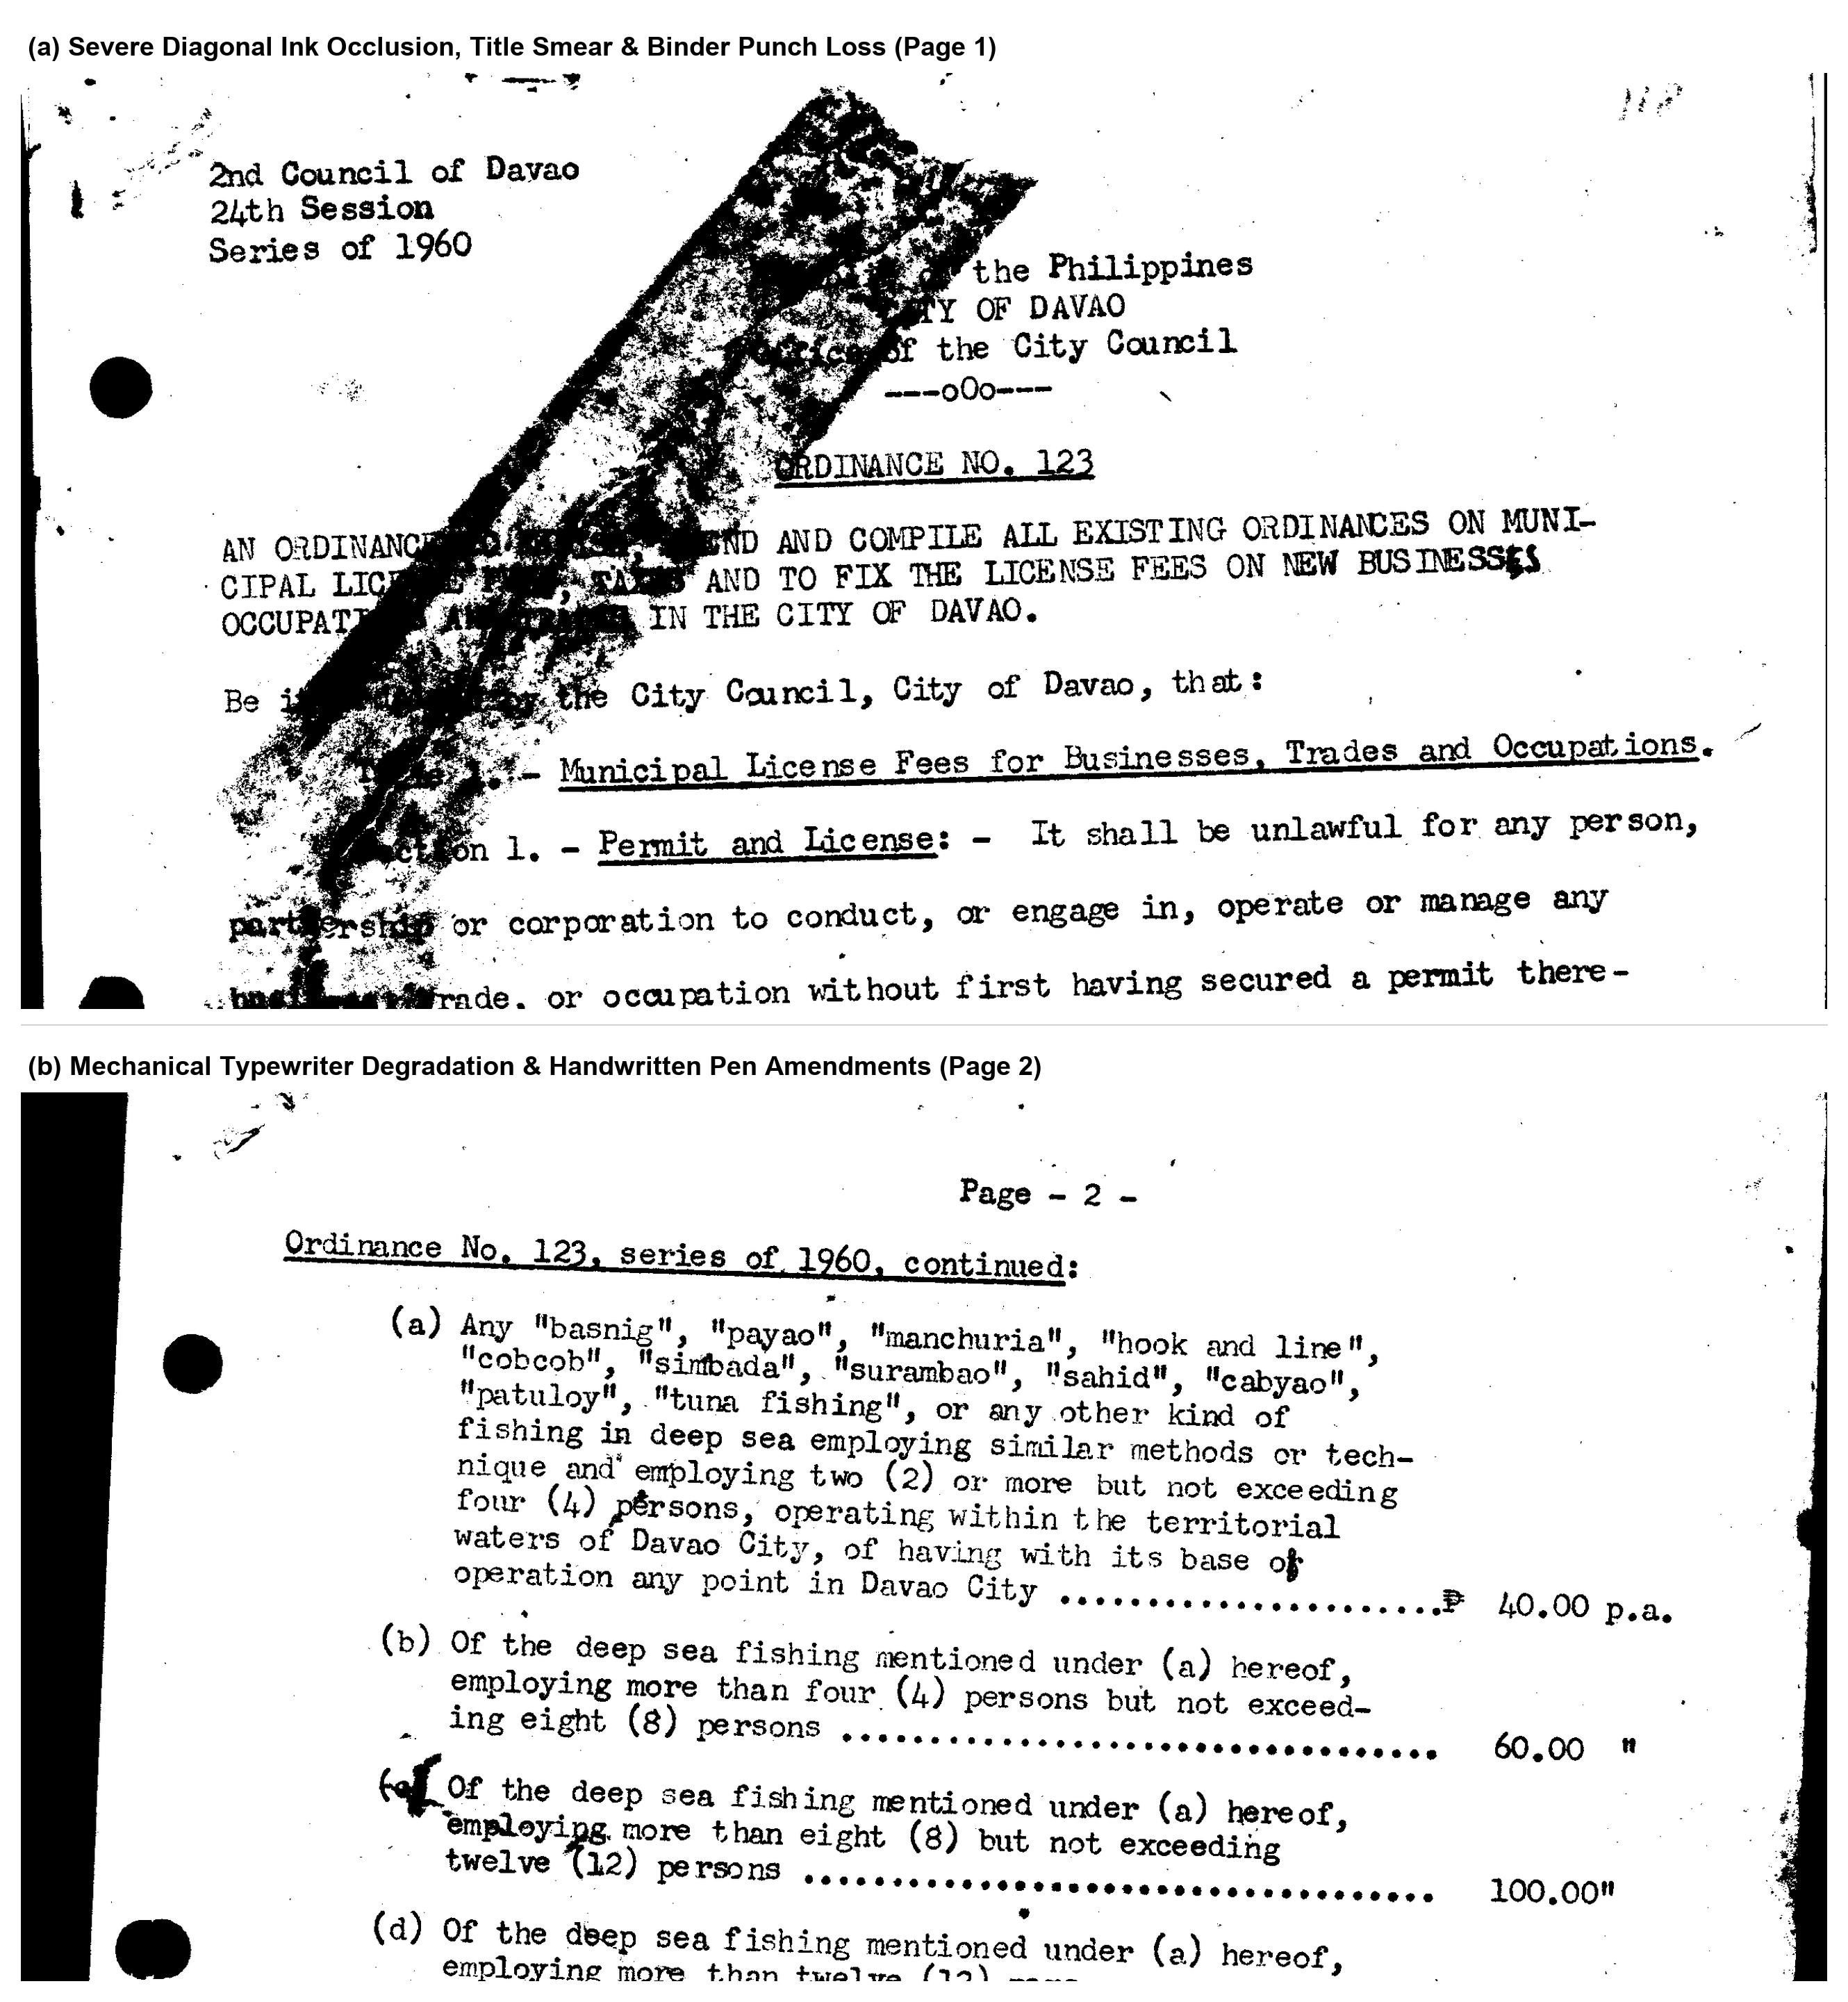
\includegraphics[width=0.88\textwidth]{figs/davao_ordinance_scan_extreme_degradation.png}
    \caption{Archival Scan Defect Plate: Historical Davao City Ordinance exhibiting mechanical typewriter ribbon exhaustion, uneven strike velocity, and paper oxidation.}
    \label{fig:app_archival_degradation_plate}
\end{figure}

Figure~\ref{fig:app_sample_ordinance_scan} displays a standard mid-era local legislative enactment from the Sangguniang Panlungsod records, highlighting structural elements such as preamble recitals, enacting clauses, and multi-column penal provisions.

\begin{figure}[htbp]
    \centering
    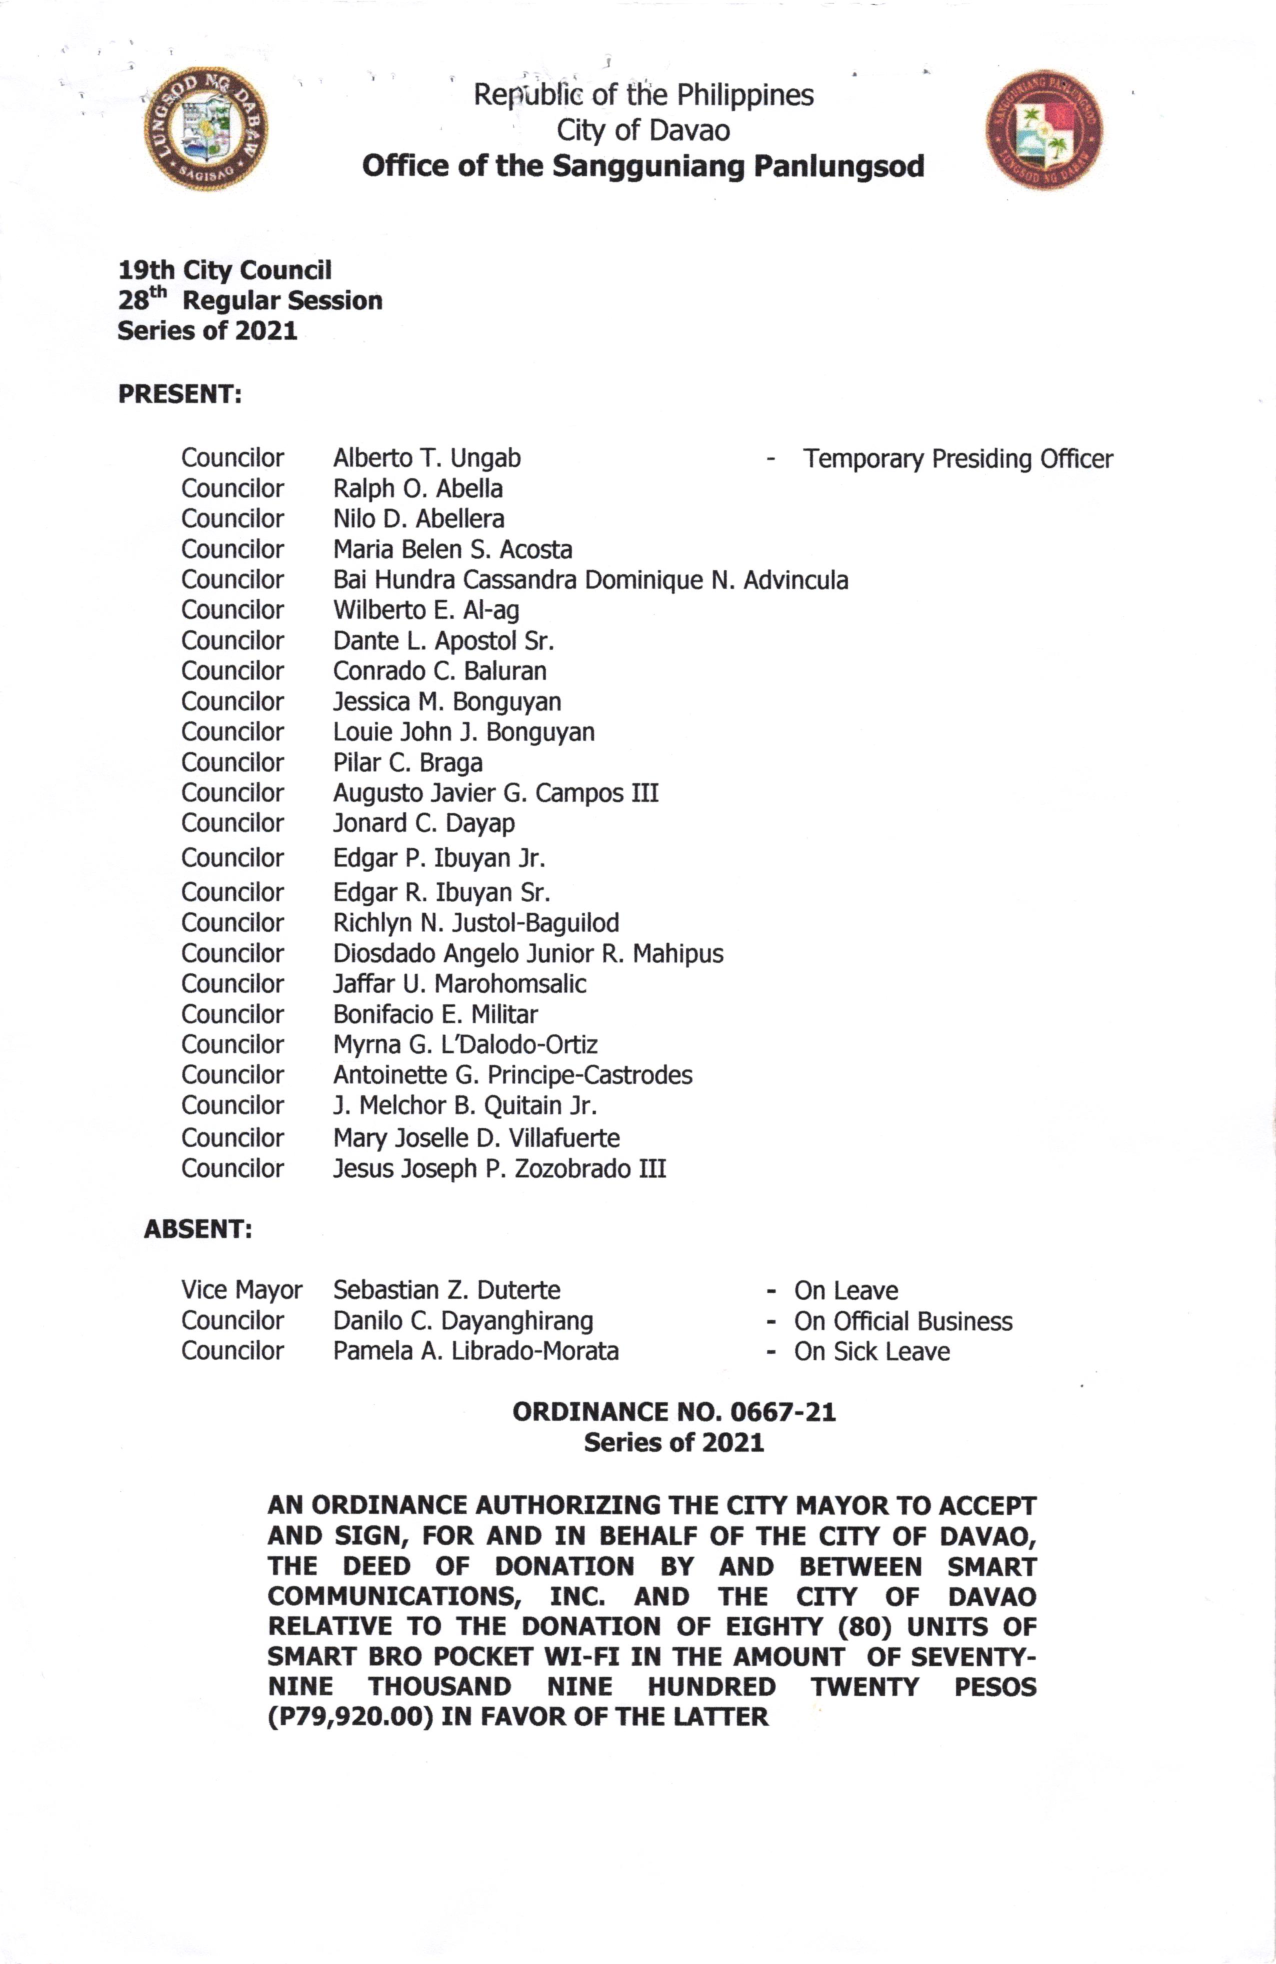
\includegraphics[width=0.82\textwidth]{figs/sample_davao_city_ordinance_scan.png}
    \caption{Representative Sangguniang Panlungsod Archival Ordinance Scan showing formal legislative preamble formatting and marginal stamp occlusions.}
    \label{fig:app_sample_ordinance_scan}
\end{figure}

\section{Comparative OCR and VLM Transcription Performance}
\label{sec:app_ocr_vlm_comparison}

To determine the most robust extraction pipeline for the 1,664 local ordinances, an empirical benchmark was conducted evaluating traditional optical character recognition engines against modern transformer-based vision and local vision-language architectures. Table~\ref{tab:app_ocr_benchmark_results} summarizes the performance across 50 representative historical pages across Character Error Rate (CER), Word Error Rate (WER), and substantive section boundary preservation.

\begin{table}[htbp]
    \centering
    \small
    \caption{Comparative OCR and Vision-Language Model Transcription Benchmark}
    \label{tab:app_ocr_benchmark_results}
    \begin{tabular}{lcccc}
        \toprule
        \textbf{Model / Engine} & \textbf{Mean CER (\%)} & \textbf{Mean WER (\%)} & \textbf{Boundary Acc. (\%)} & \textbf{Inference Speed} \\
        \midrule
        Tesseract OCR v5.4.1 (Default) & 18.42 & 27.85 & 64.2 & 0.38 s/page \\
        Tesseract OCR v5.4.1 (Bilateral + Deskew) & 11.20 & 16.48 & 76.8 & 0.52 s/page \\
        Surya OCR v0.4.15 & 7.15 & 10.92 & 84.5 & 1.84 s/page \\
        Google Cloud Vision API & 4.38 & 6.81 & 91.0 & 1.25 s/page \\
        \textbf{Qwen2.5-VL-3B-Instruct (AWQ 4-bit)} & \textbf{3.92} & \textbf{5.74} & \textbf{95.4} & 2.15 s/page \\
        \bottomrule
    \end{tabular}
\end{table}

\section{Side-by-Side Transcription Error Callouts}
\label{sec:app_ocr_transcription_callouts}

Table~\ref{tab:app_ocr_error_callouts} details characteristic transcription errors produced by traditional OCR engines on degraded archival text compared against the structured recovery achieved by vision-language modeling.

\begin{table}[htbp]
    \centering
    \scriptsize
    \caption{Side-by-Side Archival Transcription Error Examples}
    \label{tab:app_ocr_error_callouts}
    \begin{tabular}{lp{3.5cm}p{4cm}p{3.8cm}}
        \toprule
        \textbf{Archival Source} & \textbf{Verbatim Ground Truth} & \textbf{Tesseract v5.4.1 Output} & \textbf{Qwen2.5-VL-3B Output} \\
        \midrule
        Ord.~44 (1956), \S2 & \texttt{A fine of not exceeding Two Hundred Pesos (P200.00)} & \texttt{A tine of not exceedmg Two Hmxdred Pesos (P200.OO)} & \texttt{A fine of not exceeding Two Hundred Pesos (P200.00)} \\
        \addlinespace
        Ord.~332 (1968), \S4 & \texttt{shall be unlawful for any person, firm or corporation} & \texttt{shnll be unlnwful for nny person, fhm or corporntion} & \texttt{shall be unlawful for any person, firm or corporation} \\
        \addlinespace
        Ord.~166 (1981), \S1 & \texttt{Pursuant to Section 458 of the Local Government Code} & \texttt{Pmsunnt to Scction 45S of the Locnl Govemmcnt Codc} & \texttt{Pursuant to Section 458 of the Local Government Code} \\
        \bottomrule
    \end{tabular}
\end{table}
